\documentclass[a4paper, oneside, 12pt]{article}

\usepackage[utf8]{inputenc}
\usepackage[T1]{fontenc} 
\usepackage[ngerman]{babel}

\usepackage{parskip}
\usepackage{setspace}
\onehalfspacing

\usepackage[nottoc,numbib]{tocbibind}
\usepackage[bookmarks, pageanchor, hidelinks]{hyperref}
\usepackage[left=2.5cm, right=4cm, top=2.0cm, bottom=2.0cm]{geometry}

\usepackage{amsmath}
\usepackage{amsfonts}
\usepackage{graphicx}
\usepackage{subfigure}

\DeclareMathSymbol{*}{\mathbin}{symbols}{"01} % Ersetzt alle * durch \cdot in Math mode

\title{Detektion von planar aufgenommenen QR-Codes}
\author{Christian Dielitz, Simon Leistikow, Frederik Probst}

\begin{document}

\thispagestyle{empty}  % Entfernt die Seitenzahl der Titelseite
\newgeometry{top=3cm,bottom=2cm,right=3cm,left=3cm}

\hspace*{1em}
\begin{center}
	
\includegraphics[width=10cm]{images/wwu_logo}
	\par
	\vspace*{8ex}
	\Huge
	\Large\textsc{QR-Code Detektion}
	
	\vspace{10pt}
	\large Detektion von planar aufgenommenen QR-Codes
	
	\par
	\normalsize
	\vspace*{8ex}
	\normalsize
	Dokumentation zum Abschluss des\\
	\large
	\textsc{Computer Vision Praktikum}
	\par
	\normalsize
	\vspace*{12ex}
	Westfälische Wilhelms-Universität Münster\\
	Fachbereich Mathematik und Informatik\\
\end{center}
\par

\vspace*{34ex}
Eingereicht von:\\
\large
\textit{Christian Dielitz, Simon Leistikow, Frederik Probst}
\par
\normalsize
\vspace*{4ex}
Münster, 24.03.2017
\vfill
\hspace*{1em}

\newgeometry{left=2.5cm, right=4cm, top=2.0cm, bottom=2.0cm}


\newpage
\tableofcontents
\listoffigures

\newpage

\section{Einleitung}
\label{s:einleitung}
In der heutigen, digitalen Welt wird der einfache und schnelle Austausch von Informationen immer wichtiger. Als eines von vielen Kommunikationsträgern dient dabei der sogenannte Quick Response (kurz QR) Code, da er Informationen gut komprimieren und durch bestimmte Software schnell wieder zurück verarbeitet werden kann.

Ein QR-Code ist im wesentlichen ein Raster von schwarzen und weißen Flächen, welche Quadratisch angeordnet sind. In aktuelleren Standards ist es allerdings auch erlaubt, kleinere Bilder (wie z.B. Firmenlogos) in den QR-Code zu integrieren. Heutzutage sind QR-Codes sehr populär und werden meist zur Kodierung von Internetseiten verwendet. Der Einsatzbereich eines QR-Codes beschränkt sich allerdings nicht nur auf URL Komprimierung: Mit seiner Hilfe lässt sich jeder beliebige Text, Bilder oder sogar Hologramme kompakt darstellen. Ein wesentliches Problem von QR-Codes ist allerdings, dass nicht direkt ersichtlich ist, welche Daten ein QR-Code enthält. Beispielsweise wäre es möglich Schadsoftware zu kodieren, welche beim Lesen ausgeführt wird und das entsprechende Lesegerät befällt.

Da die Eingabe eines QR-Codes meist durch ein aufgenommenes Bild einer Kamera vorliegt, ist es unumgänglich, dass eine schnelle Lokalisierung und Transformation in einen lesbaren Zustand des QR Codes durchgeführt werden muss.

Innerhalb diese Praktikums haben wir uns damit auseinander gesetzt, wie man planar aufgenommene QR-Codes möglichst schnell und zuverlässig aus einem Bild extrahieren kann. Dazu haben wir, basierend auf OpenCV, ein Programm entwickelt, welches sowohl Bilder von der Webcam eines Computers aufnehmen als auch schon gespeicherte Bilder laden kann und den  darin enthaltenen QR Code als eigenständiges Bild extrahiert.

\section{Aufgabenstellung}
\label{s:aufgabenstellung}
Die offiziell, wortgetreue Aufgabenstellung lautete dabei wie folgt:

Schreiben Sie ein Programm, welches ein Eingabebild entgegennimmt und in diesem (wenn möglich) einen planar aufgenommenen QR-Code lokalisiert und als binarisiertes Bild ausgibt. Sollte kein QR-Code im Bild lokalisiert werden können, so geben Sie ein $1 \! \times \! 1$ Pixel großes, schwarzes Bild aus. Gehen Sie davon aus, dass in jedem Bild maximal ein QR-Code enthalten ist.


\newpage

\section{Grundlagen}
\label{s:grundlagen}

\subsection{Aufbau eines QR-Codes}
\label{ss:aufbau}

Ein QR-Code in eine Matrix $M = n \times n$ \Big(auf Grund der aktuellen Standards gilt $n \in \big\{17+4*v \,\, | \,\, v \in  \{1,\dots, 40\}\big\}$\Big) welche die kodierten Daten in Binär Form darstellt. Ein schwarzes Quadrat stellt dabei eine 1 dar und ein leeres, weißes Feld eine 0.

\begin{figure}[h]
	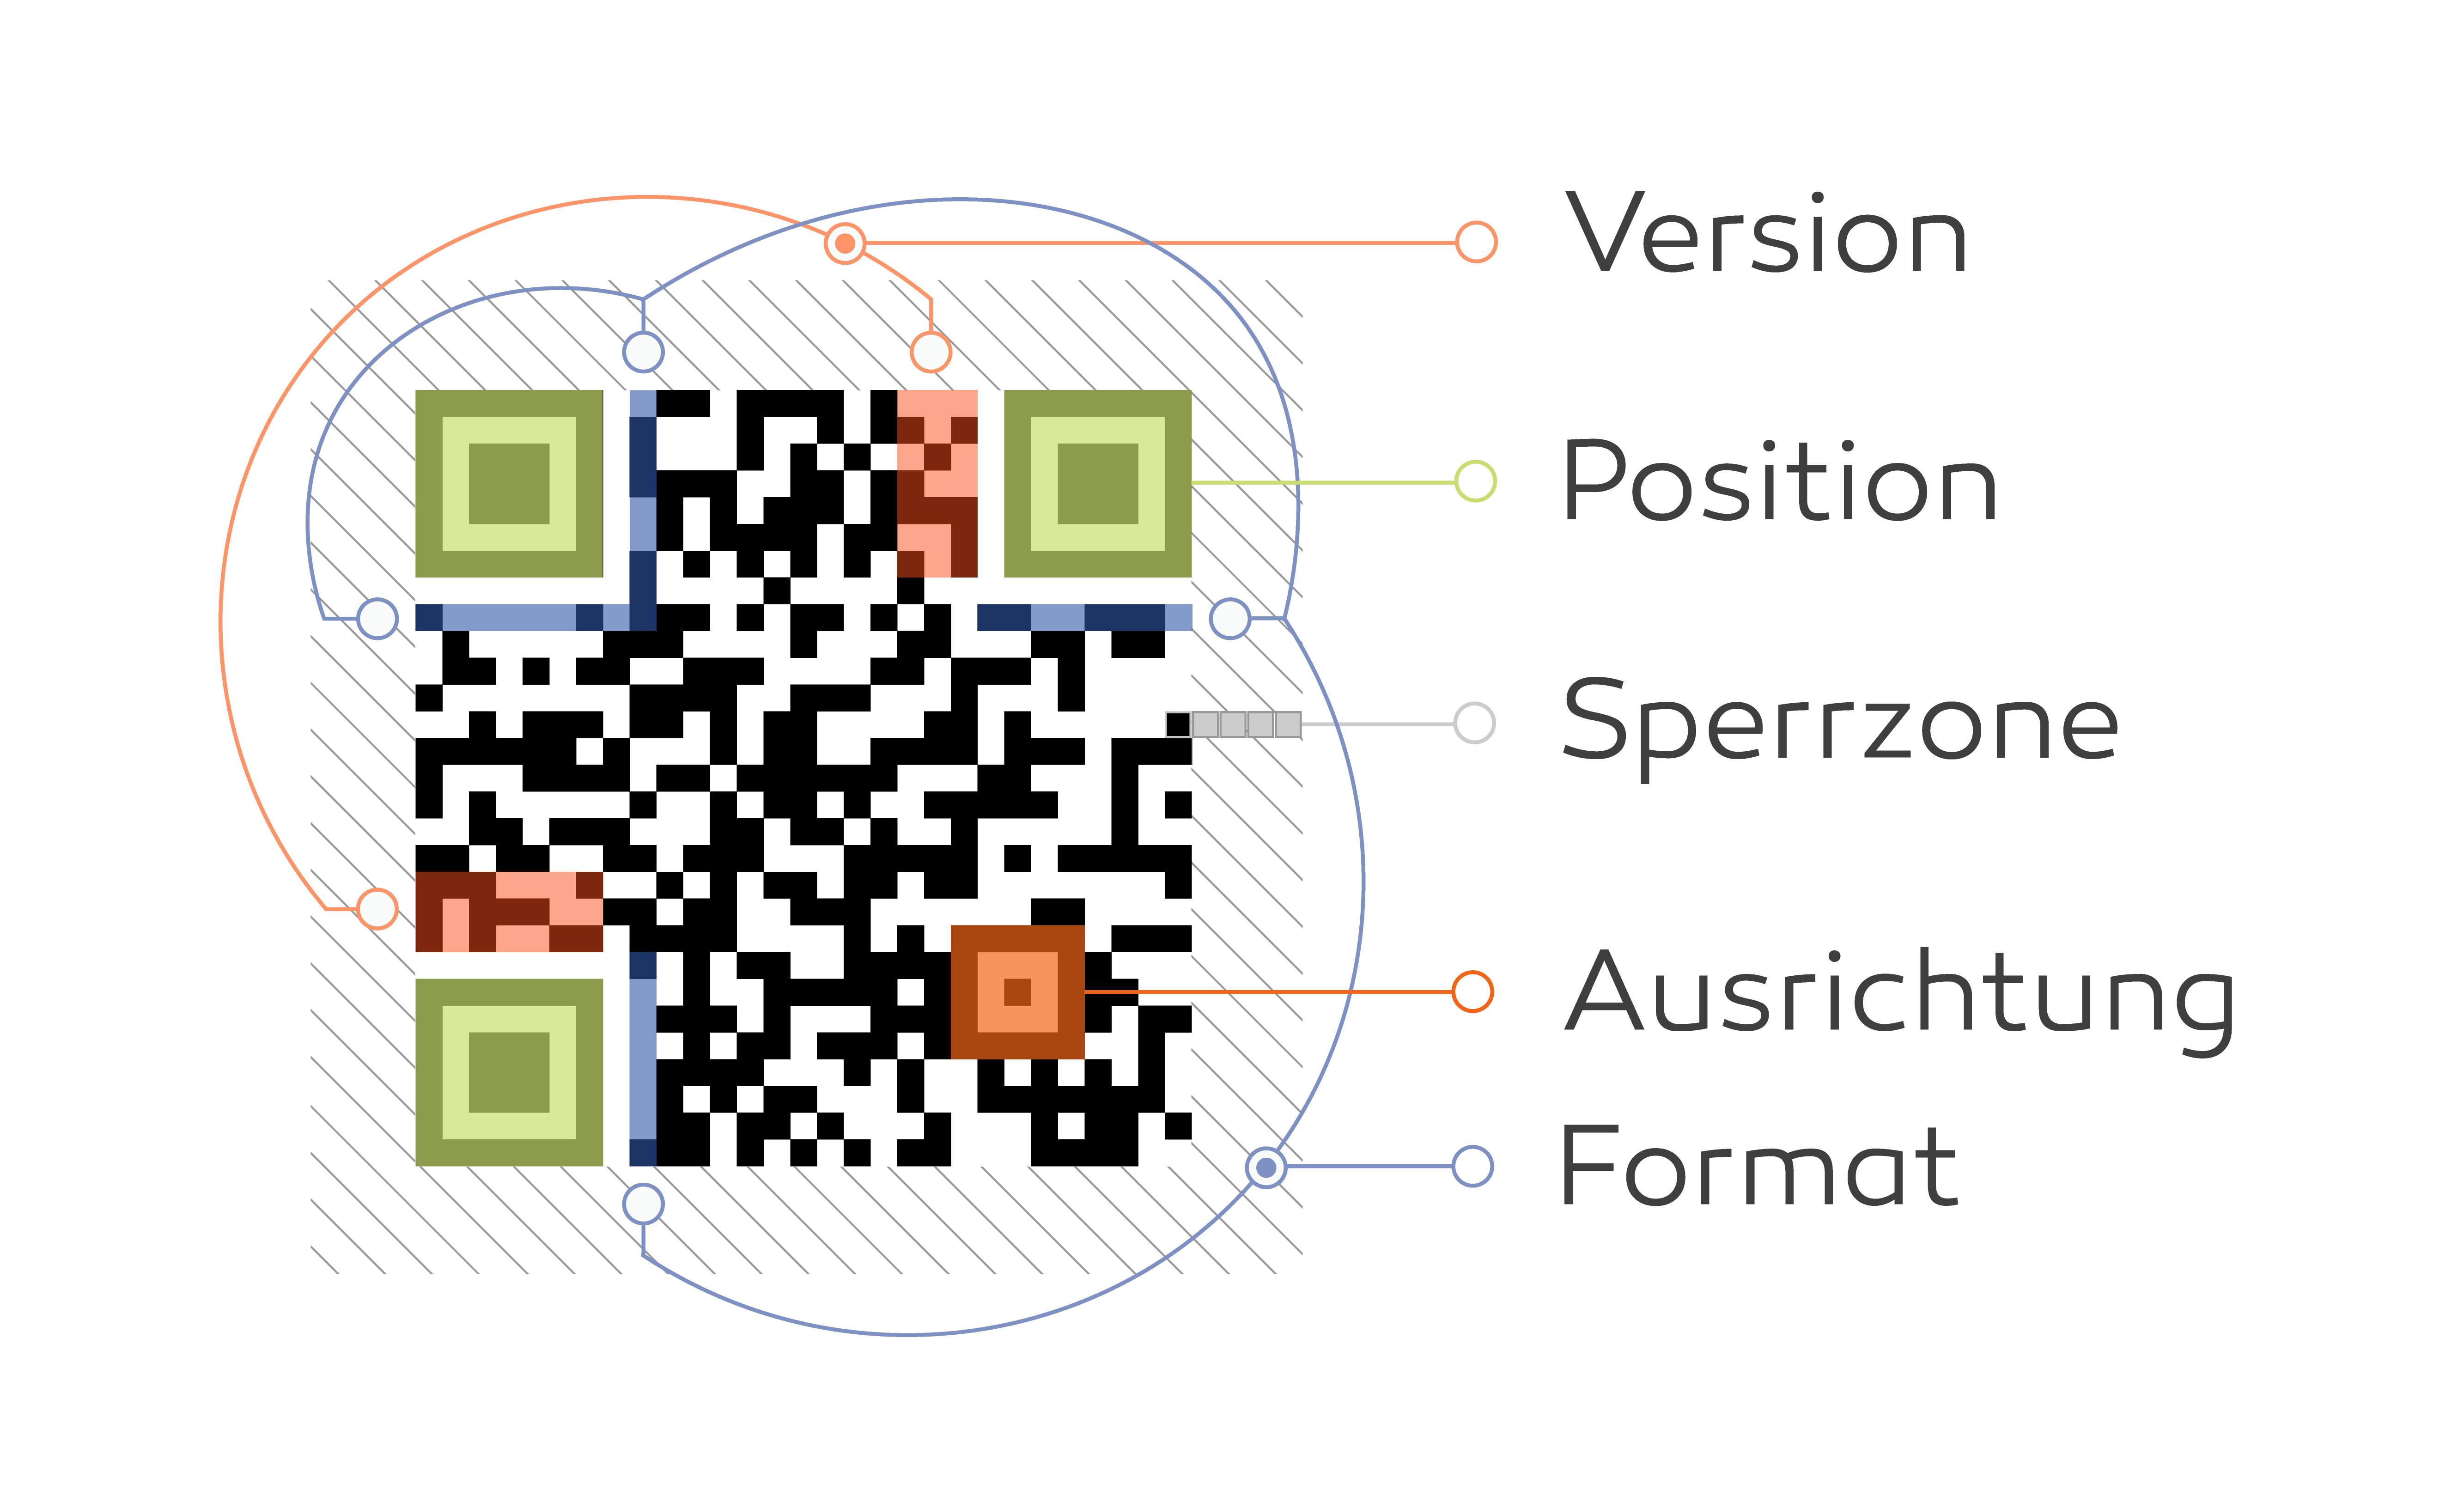
\includegraphics[width=\textwidth]{images/aufbau.png}
	\caption{Aufbau eines Beispiel QR-Codes}
	\label{fig:aufbau}
\end{figure}

Die in Abbildung \ref{fig:aufbau} grün markierten Quadrate sind die Positionsmarker des QR-Codes. Durch sie ist die Ausrichtung und Position eindeutig festgelegt. Außerdem ist es mit Ihrer Hilfe möglich, den vierten Eckpunkt zu bestimmen. Sie sind genau 8 Module Groß und der äußere, weiße Rand, sowie der Abstand vom inneren zum äußeren Quadrat ist genau 1 Bit breit.

Am äußeren Rand der Positionsmarker verläuft das sogenannte Timing-Pattern, welches abwechselnd aus schwarzen und weißen Modulen besteht. Es dient einzig zur vereinfachten Bestimmung der Positionsmarker und kann für eine spätere Transformation hilfreich sein.

Direkt an die Positionsmarker oben rechts und unten links grenzen die Versionsinformationen an,  welche durch die roten Flächen gekennzeichnet sind. Sie beschreiben die verwendete Version des QR Codes, welche wiederum die Größe des QR-Code festlegt. In der zuletzt erschienenen Version 40 ist, durch die oben beschriebene Formel, eine maximale Größe von $177 \times 177$ Datenpunkten erlaubt.

An der jeweils anderen Seite der beiden Positionsmarker und zusätzlich an beiden Seiten vom Positionsmarker oben links ist das jeweilige Format des QR-Codes dargestellt (blaue Streifen in Abbildung \ref{fig:aufbau}). Die Streifen sind jeweils genau ein Bit Breit und enthalten Informationen über das Fehlerkorrektur-Level und das verwendete Masken-Pattern um den QR Code zu kodieren.% Diese Eigenschaften werden in Kapitel \ref{ss:fehlerkorrektur} und \ref{ss:codierung} noch genauer  betrachtet.

Jeder QR-Code ist von einer sogenannten Sperrzone umgeben, welche komplett weiß sein muss. Diese Pixel enthalten noch keine Informationen über die kodierten Daten und dienen zur Freilegung der Positionsmarker, was für die Konturerkennung notwendig ist. Die Sperrzone umfasst den gesamten QR-Code und ist an jeder Stelle gleich Breit.

Ab Version 2 wurden außerdem zusätzliche Ausrichtungsmarker eingeführt, welche die Berechnung der Position noch einmal vereinfachen sollen. Sie sind deutlich kleiner (jeweils 5 Module in Länge und Breite) als die eigentlichen Positionsmarker und können dem QR-Code optional hinzugefügt werden.

Beachtet man all diese Formalien, so ist es mit folgender Formel möglich, den Speicherplatz eines QR-Codes zu berechnen:
\begin{align*}
&size &&= (17 + 4 * v)^2 \hspace{200pt} | \,\, v \in 1,\dots,40\\
&info &&= Position + Ausrichtung + TimingPattern + Format + Version\\
&bits &&= size - info
\end{align*}

Im Falle der aktuellsten Version 40 mit einem Fehlerkorrekturlevel L (7\%) ist also eine Kodierung von $23648$ Bits möglich.

%\subsection{Fehlerkorrektur}
%\label{ss:fehlerkorrektur}

%\subsection{Codierung der Daten}
%\label{ss:codierung}

\subsection{Globales Thresholding nach Otsu}
\label{ss:otsu}

Ein Bild zu binearisieren bedeutet, seine Pixel genau einer von zwei Klassen zuzuordnen. Für dieses Problem gibt es verschiedene Lösungsansätze wie zum Beispiel das globalen Thresholding. Bei dieser Methode wird jeder einzelne Pixel des Bildes $I$ gegen einen konstanten Wert $t$ verglichen. Ist $I_{r,c} \leq t$, so wird dieser Pixel der ersten Klasse zugewiesen, andernfalls der zweiten Klasse.

Bei Bildern mit verschiedenen Helligkeitsbereichen versagt diese Methode jedoch recht schnell und oftmals ist ein geeigneter Trasholding Wert nicht bekannt. Genau diese Problematik versucht die Otsu Methode zu umgehen, indem sie den optimalen Wert für ein globales Thresholding dynamisch berechnet. Die Idee des Verfahrens ist, im Grauwerthistogramm des Bildes nach zwei Peaks zu suchen und dessen Mitte als Thresholding Wert zu verwenden. Aus diesem Grund eignet sich die Otsu Methode besonders gut für Bilder, welche im wesentlichen nur aus zwei Hauptfarben bestehen.

Ziel der Binarisierung ist es so wenig Pixel wie möglich der falschen Klasse zuzuordnen. Im Kontext der beiden Peaks heißt das, dass deren Streuung sich nicht überschneiden aber trotzdem den ganzen Farbbereich abdecken sollte. Ein Maß für die Streuung ist die Varianz, mit welcher sich folgendes Minimierungsproblem formulieren lässt: $\sigma^2(t) = q_1 * \sigma^2_1(t) + q_2 * \sigma^2_2(t)$
\begin{align*}
	&q_1(t) = \sum_{i=1}^{t} P(i)
	&&q_2(t) = \sum_{i=t+1}^{I} P(i)\\
	&\mu_1(t) = \sum_{i=1}^{t} \frac{i * P(i)}{q_1(t)}
	&&\mu_2(t) = \sum_{i=t+1}^{I} \frac{i * P(i)}{q_2(t)}\\
	&\sigma^2_1(t) = \sum_{i=1}^{t} [i - \mu_1(t)]^2 * \frac{P(i)}{q_1(t)} \hspace{50pt}
	&&\sigma^2_2(t) = \sum_{i=t+1}^{I} [i - \mu_2(t)]^2 * \frac{P(i)}{q_1(t)}
\end{align*}

Hierbei entsprechen $\mu_1$ und $\mu_2$ genau der Definition des Erwartungswertes; das selbe gilt für $\sigma_1$ und $\sigma_2$ im Bezug auf die Varianz. Da das Histogramm allerdings bei $t$ aufgeteilt wird, müssen die Wahrscheinlichkeiten durch die Division korrigiert werden.

Gesucht ist nun der Wert $t$, für welchen $\sigma^2(t)$ minimal wird. Es müssen also 256 (Anzahl möglicher Splits im Grauwerthistogramm) Werte für $t$ getestet werden, bis der optimale Thresholding Wert gefunden wurde.

\begin{figure}[h]
	\centering
	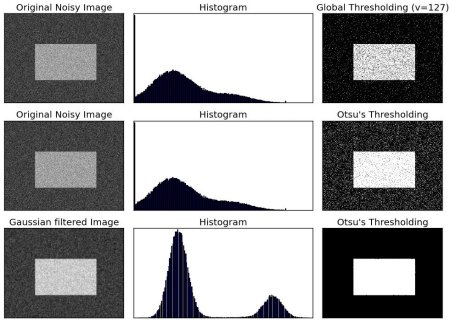
\includegraphics[width=0.7\textwidth]{images/otsu.jpg}
	\caption{Vergleich von Thresholding Verfahren}
	\label{fig:otsu}
\end{figure}

Wie in Abbildung \ref{fig:otsu} zu sehen, können durch die Kombination von Gaußfilter und Otsu Thresholding sehr gute Ergebnisse für (größtenteils) zweifarbige Bilder entstehen. Durch die vorherige Suche des Thresholding Werts dauert dieses Verfahren allerdings auch etwas länger.

% Hier bitte einmal kurz erklären, wie der Funktioniert, gerne auch mit Bildern.
% Siehe: http://docs.opencv.org/3.2.0/d7/d4d/tutorial_py_thresholding.html
% Abschnitt: How Otsu's Binarization Works?

\newpage

\section{Implementierung}
\label{s:implementierung}

Die wesentliche Aufgabe des Praktikums war es, die recherchierten Grundlagen (siehe Kapitel \ref{s:grundlagen}) zu verwenden, um einen lauffähigen QR-Code-Detektor zu implementieren. Dessen Ein- sowie Ausgabe werden im Folgenden näher definiert.
Im Anschluss wird auf Details der Detektion eingegangen und erklärt, wie die Ausgabe aus der Eingabe gewonnen wird.
Grundsätzlich arbeitet das Programm in zwei Modi: dem \emph{Release}- und dem \emph{Live}-Modus.
Ersterer ist für die Evaluierung erstellt worden und erzeugt ein reines Konsolenprogramm, welches ohne weitere Umwege die Eingabe in die Ausgabe überführt.
Im \emph{Live}-Modus hingegen verwendet das Programm die Webcam des ausführenden Rechners als Eingabe, falls vorhanden. Es werden also, abhängig von deren Aufnahmeeigenschaften, kontinuierlich neue Eingaben und somit Ausgaben generiert. Dabei werden zusätzliche visuelle Ausgaben der durchgeführten Zwischenschritte erzeugt, welche im Unterkapitel \ref{s:detektion} näher erläutert werden.
Die Implementierung ist in \emph{C++} \cite{stroustrup1995c++} in Verbindung mit \emph{OpenCV} \cite{bradski2008learning} als Algorithmenbibliothek geschrieben.

\subsection{Eingabe}
\label{s:eingabe}

Als Eingabe für das im Rahmen des Praktikums erstellte Programm dient ein Bild in üblichem, d. h. von OpenCV lesbarem, Format. Als Beispiele seien hier \emph{JPG}, \emph{PNG} und \emph{BMP} genannt.
Dies darf nach Aufgabenstellung höchstens einen QR-Code enthalten.
Desweiteren schränken wir die Eingabe ein, indem wir höchstens drei \emph{Finder-Pattern} erkennen.
Im Falle des \emph{Live}-Modus generiert die verbundene Webcam die Eingabebilder.

\subsection{Ausgabe}
\label{s:ausgabe}

Die Ausgabe des Programms lässt sich erneut nach den beiden Modi aufteilen.
Im \emph{Release}-Modus wird genau ein Bild gemäß Aufgabestellung (siehe Kapitel \ref{s:aufgabenstellung}) erstellt. Letztlich soll jedoch unterschieden werden, ob der QR-Code im Eingabebild erkannt werden konnte oder nicht. Im Falle eines Fehlers wird ein 1x1 Pixel großes, schwarzes Bild generiert. Bei erfolgreicher Detektion hingegen ein quadratisches Bild, deren Dimension exakt der des QR-Codes im Eingabebild entspricht.
Ein QR-Code mit 29x29 Modulen im Eingabebild erzeugt somit ein Ausgabebild der Größe 29x29 Pixeln, wobei die Farbe eines Pixels exakt dem Wert eines Moduls entspricht.
Das Bild wird verlustfrei im \emph{PNG}-Format gespeichert, um möglichen Datenverlust zu verhindern.
Im \emph{Live}-Modus hingegen wird keine Datei, sondern lediglich visuelle Ausgabe erzeugt. Das Ergebnis wird in einem Fenster angezeigt und kann direkt betrachtet werden. Auf weitere Details wird im folgenden Kapitel eingegangen.

\subsection{Detektion}
\label{s:detektion}

Der Begriff der Detektion lässt sich unmittelbar aus der Problemstellung herleiten.
Gefordert ist insbesondere nicht das Lesen des QR-Codes, sondern lediglich das Verorten und Normalisieren des QR-Codes, bzw. das Feststellen von dessen Abwesenheit im Bild. Die dafür notwendigen Schritte werden in den Unterkapiteln dieses Kapitels erläutert.

\subsubsection{Vorverarbeitung}
Die Vorverarbeitung spielt in der Bildverarbeitung meist eine große Rolle. Die Qualität von Echtweltdaten ist oftmals weit entfernt vom Optimum, sodass die Anwendung eines Algorithmus auf diesen im Allgemeinen keine oder nur dürftige Ergebnisse liefert.
Dies trifft auch auf die gegenwärtige Problemstellung zu. Eingabebilder, insbesondere durch eine Webcam erzeugte, können mehrere Probleme aufweisen.
Geläufige Beispiele sind hierbei Rauschen, Verwaschungen und Unschärfe, welche durch den Sensor der Kamera, schlechte Lichtverhältnisse oder eine unruhige Kameraführung entstehen können. Ebenfalls kann es zu Spiegelungen und Reflektionen kommen, wenn  der QR-Code beispielsweise auf einem Handydisplay angezeigt wird.

\begin{figure}[h]
	\begin{center}
		\subfigure[Eingabebild]{
			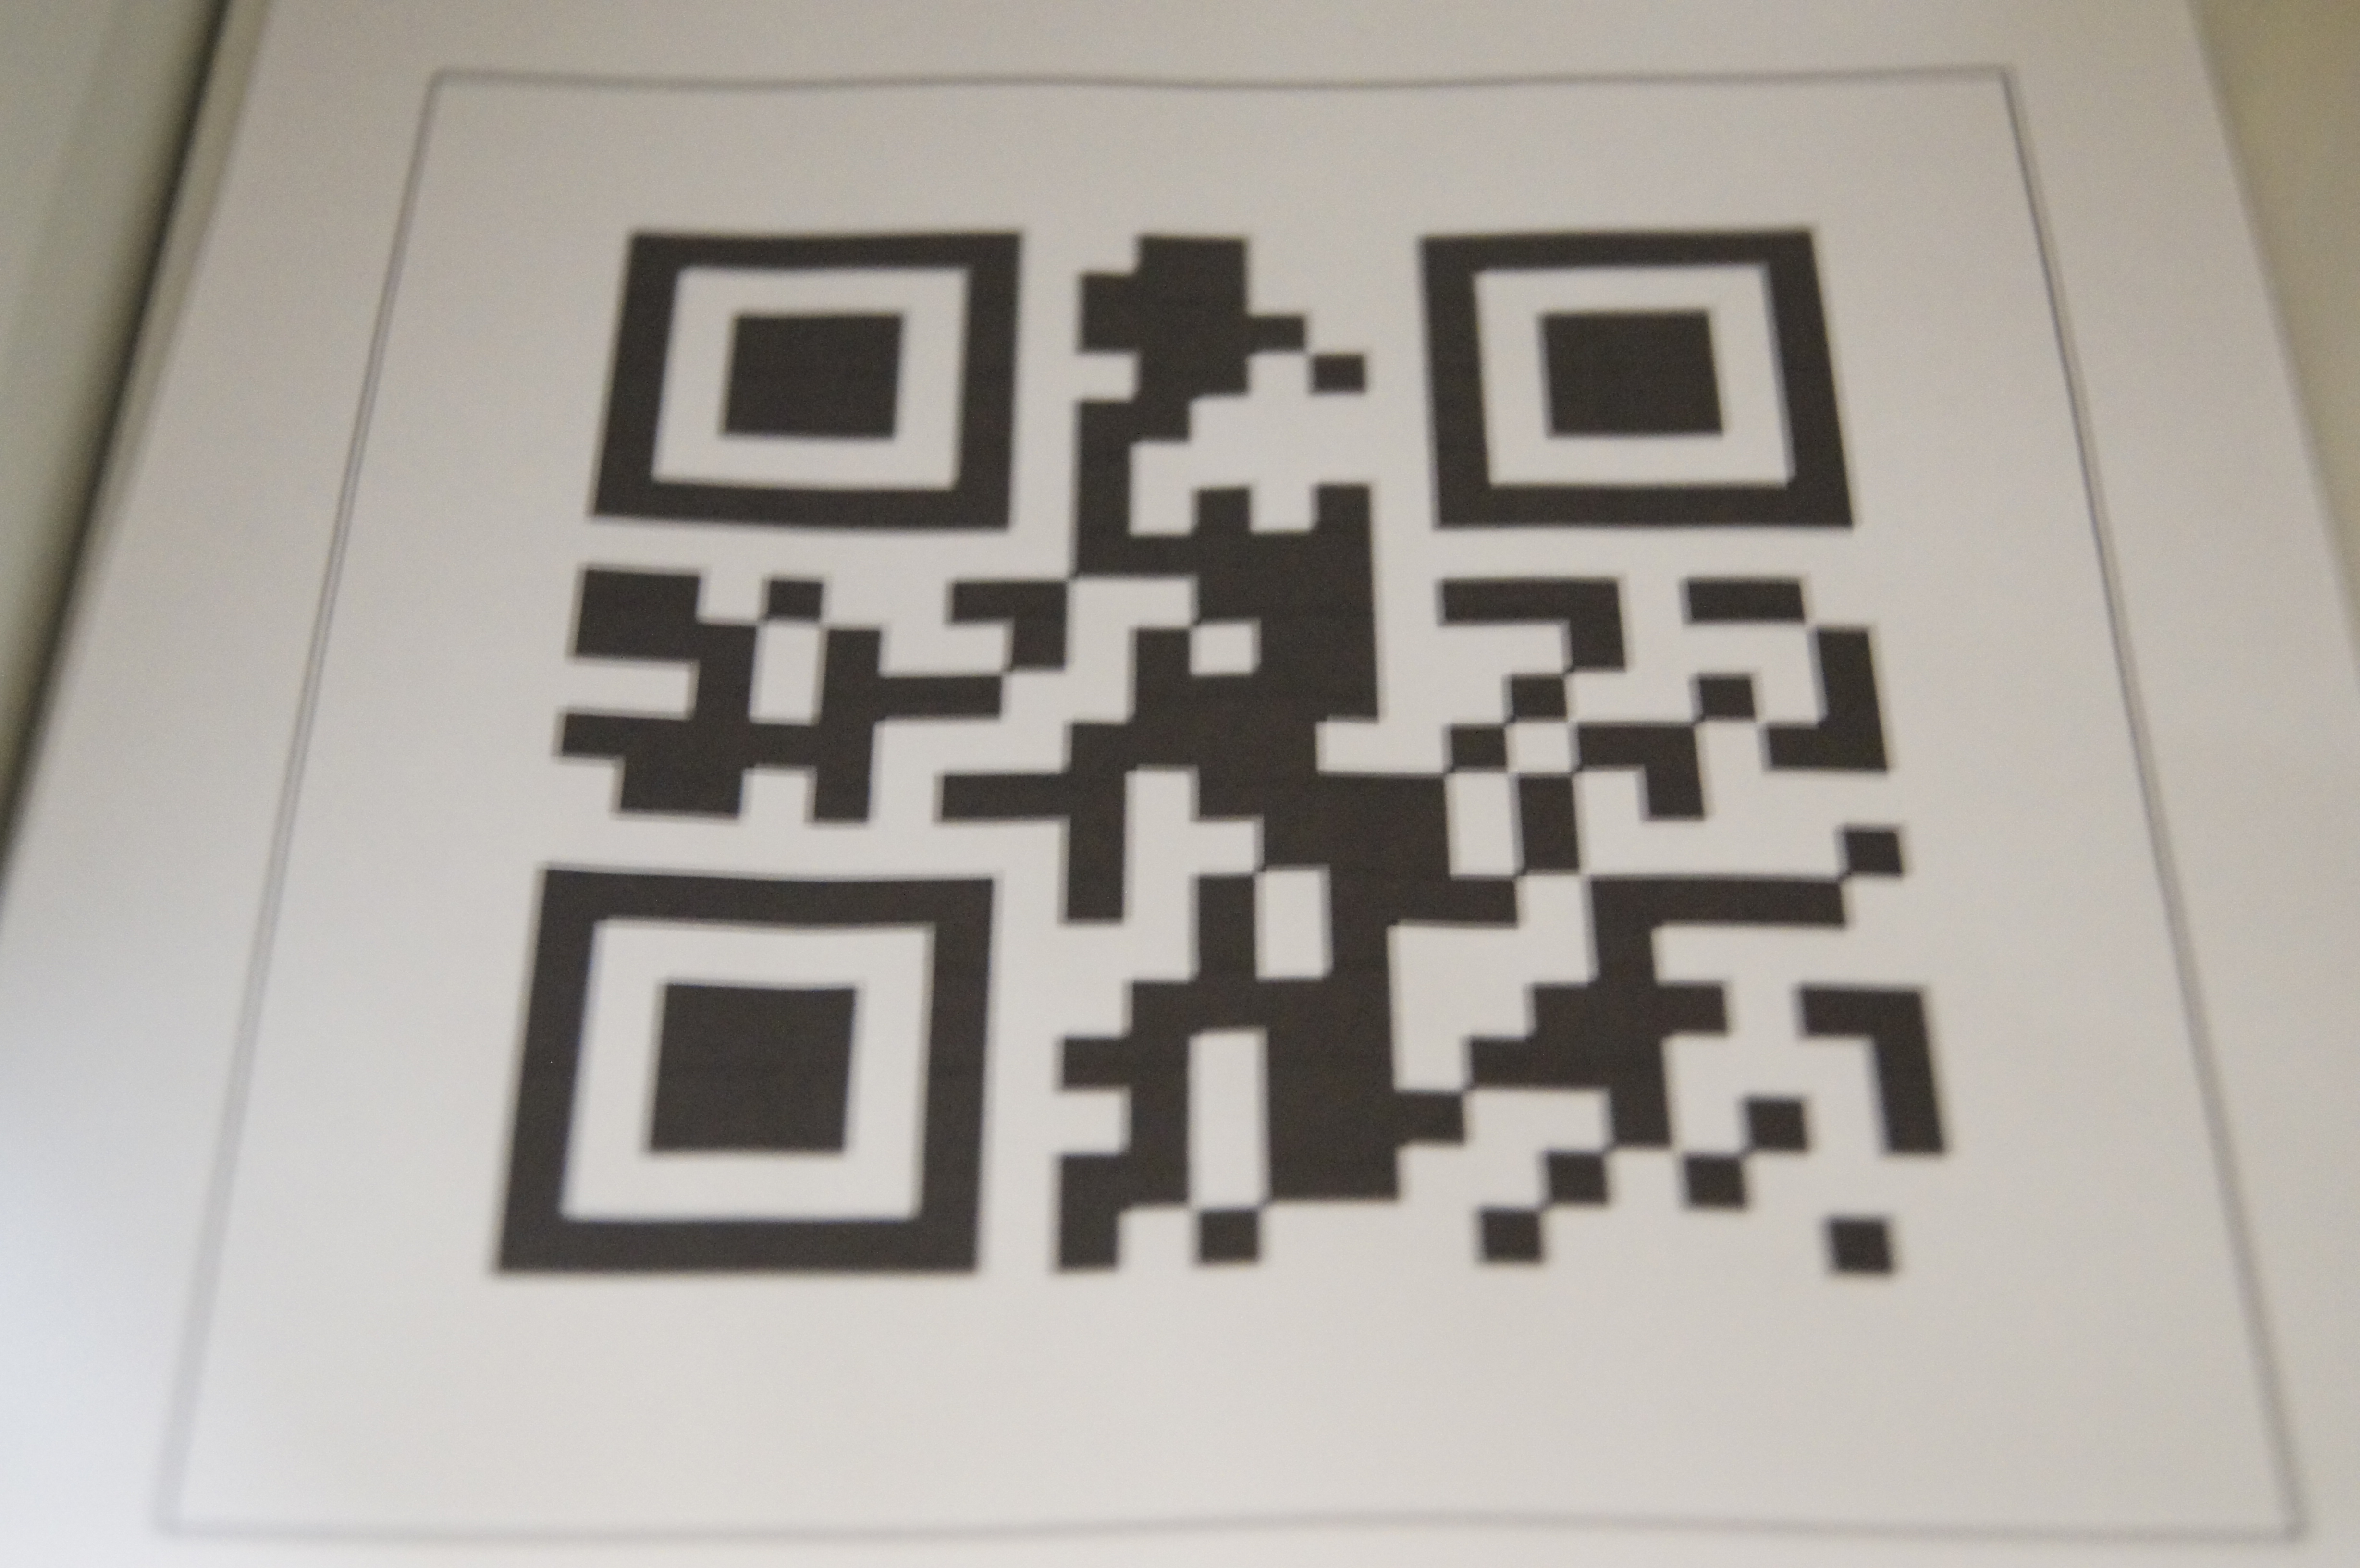
\includegraphics[width=0.45\linewidth]{./images/original.jpg}
			\label{fig:eingabebild}
		}
		\subfigure[binarisiertes und gefiltertes Bild]{
			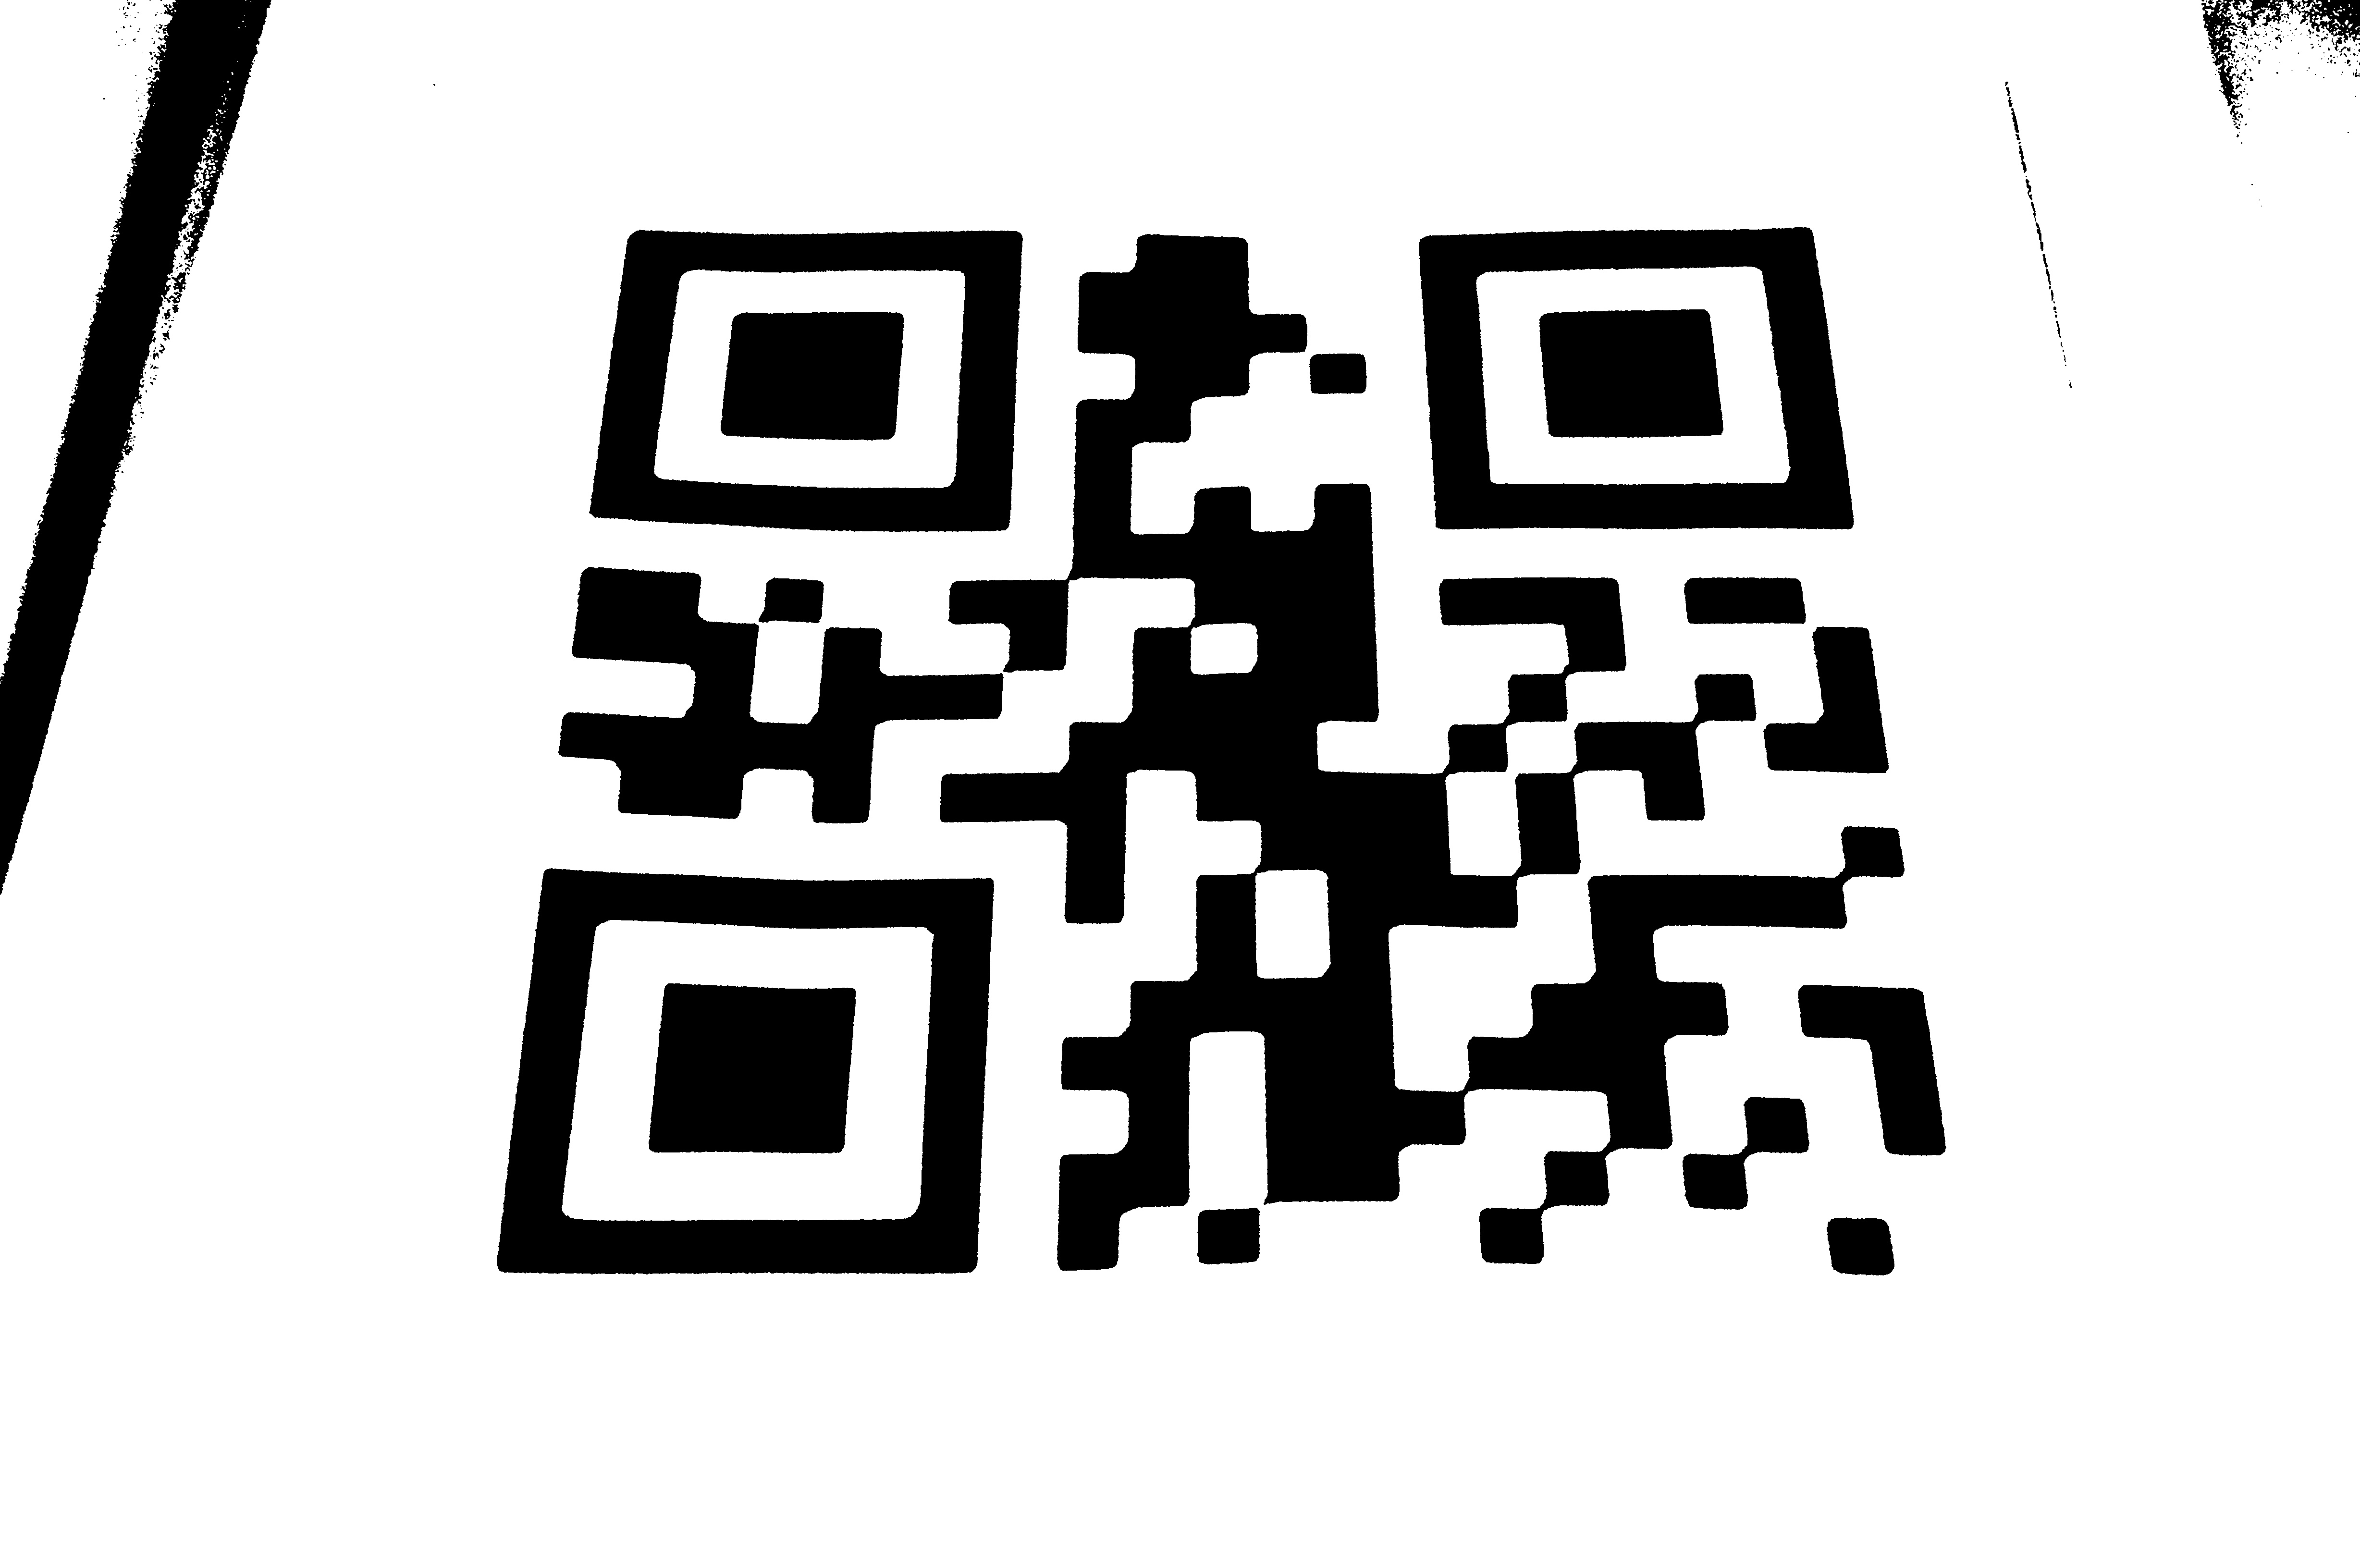
\includegraphics[width=0.45\linewidth]{./images/gray.jpg}
			\label{fig:binarisiert}
		}
	\end{center}
	\caption{Die Zusammenfassung der Vorverarbeitungsschritte.}
	\label{fig:vorverarbeitung}
\end{figure}

Um diese Probleme zu reduzieren und die Erkennung möglichst stabil zu gestalten, wird die Eingabe (siehe Abbildung \ref{fig:eingabebild}) zunächst in ein Graustufenbild umgewandelt, was im Wesentlichen durch die Anwendung der folgenden Schritte begründet ist.
Es folgt eine Anwendung des Medianfilters in einer Achter-Nachbarschaft, welche Rauschen und Verwaschungen minimieren kann. Die Wahl der Nachbarschaftsgröße wurde anhand eigener Testdaten experimentell ermittelt (siehe Kapitel \ref{s:evaluierung}).
Als nächstes wird das gefilterte Graustufenbild binarisiert, was den Kontrast des QR-Codes im Bild maximiert. Diese Eigenschaft ist für die nachfolgende Kantendetektion eine wichtige Bedingung.
Zum Abschluss wird erneut der Medianfilter angewendet, da dies zu einer weiteren Verbesserung der Erkennungsquote führt.
Das Ergebnis der Vorverarbeitung ist in Abbildung \ref{fig:binarisiert} zu sehen.

\subsubsection{Lokalisierung}

Bei der Lokalisierung geht es um die Verortung des QR-Codes, d.h. die Bestimmung dessen Positionsmarker. Dafür wird nun nicht mehr das Eingabebild selbst, sondern das Ergebnis der Vorverarbeitung verwendet.
Grund dafür ist, dass der \emph{Canny}-Operator \cite{canny1986computational} auf das Bild angewendet wird, um die enthaltenen Konturen zu erhalten, welcher gut bei hohem Konstrast bzw. bei scharfen Kanten funktioniert. Im Detail bedeutet dies, dass die Wahl der Grenzwerte der enthaltenen Hysterese-Operation recht flexibel ausfällt. Ausgehend von einer maximalen Kantenstärke von 255 haben wir uns für eine untere Schwelle von 50 und eine obere Schwelle von 180 entschieden, da diese Werte im Vergleich zu keiner Verschlechterung unserer Testergebnisse geführt haben. Es sei jedoch erwähnt, dass auch Werte von 20 bzw. 150 das Ergebnis nicht beeinflusst haben, was die Flexibilität in der Wahl der Parameter unterstreicht, welche durch die scharfen Kanten erreicht wurde.

\begin{figure}[h]
	\begin{center}
		\subfigure[Ergebnis einer Kantendetektion]{
			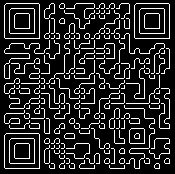
\includegraphics[width=0.45\linewidth]{./images/edges.jpg} %TODO: besseres Bild
			\label{fig:canny}
		}
		\subfigure[Hierarchie der Konturen eines Positionsmarkers]{
			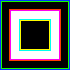
\includegraphics[width=0.45\linewidth]{./images/area.png}
			\label{fig:konturen}
		}
	\end{center}
	\caption{Das Ergebnis der Kantendetektion eines QR-Codes und der Konturerkennung.}
	\label{fig:lokalisierung}
\end{figure}

Im nächsten Schritt werden die Konturen samt ihrer Hierarchie aus den gewonnenen Kantenstärken extrahiert. Gesucht werden dabei Konturen, welche exakt fünf ineinandergeschachtelte Konturen enthalten. Zu dieser Einschränkung kommt es durch die Arbeitsweise der verwendeten Bibliothek und durch den Aufbau der Positionsmarker der QR-Codes. Letztere bestehen aus 7x7 Modulen in quadratischer Anordnung und sind durch eine weiße Sperrschicht umgeben (siehe Kapitel \ref{ss:aufbau}). Durch den weißen Bereich im Innern ergeben sich somit drei Farbwechsel über den halben Querschnitt, welche jeweils doppelt gezählt werden, da sowohl der Wechsel von außen nach innen, als auch der Wechsel von innen nach außen gezählt wird, was in Abbildung \ref{fig:konturen} zu erkennen ist. Wir suchen letztlich die blau markierte Kontur, da diese den größten Umfang hat, was bei der geometrischen Normalisierung im folgenden Unterkapitel von Bedeutung sein wird.

An dieser Stelle ist jedoch ein weiteres Kriterium zum Erkennen der Positionsmarker notwendig, da die Verschachtelung der Konturen kein Alleinstellungsmerkmal ist.
Betrachten wir hingegen zusätzlich die Verhältnisse der Flächeninhalte hierarchisch aufeinanderfolgender Konturen, so stellt sich dies als recht sicheres Erkennungsmerkmal heraus. Durch die bekannte Einteilung des Positionsmarkers in Module lässt sich, von außen nach innen betrachtet, die Abfolge $1 - 7^2:5^2 - 1 - 5^2:3^2 - 1$ der Verhältnisse von jeweils äußerer zu innerer Kontur festhalten.
Diese Verhältnisse bleiben auch bei perspektivischer Verzerrung in etwa bestehen, wobei ein Schwellwert auch hier etwaigen Ungenauigkeiten Abhilfe verschafft.
Zusammengenommen stellen diese beiden Kriterien bereits einen guten Klassifikator für Positionsmarker dar. Sollten dennoch mehr als drei Treffer gefunden werden, bricht das Programm ab, da von mehr als einem QR-Code im Eingabebild auszugehen ist.

\subsubsection{Geometrische Normalisierung}

\begin{figure}[t]
	\begin{center}
		\subfigure[Orientierung eines QR-Codes]{
			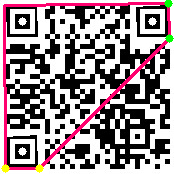
\includegraphics[width=0.45\linewidth]{./images/bounds.jpg}
			\label{fig:orientierung}
		}
		\subfigure[Darstellung einer perspektivischen Transformation]{
			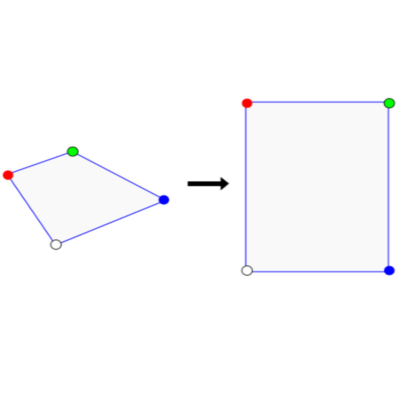
\includegraphics[width=0.45\linewidth]{./images/perspective.jpg}
			\label{fig:perspektivisch}
		}
	\end{center}
	\caption{Darstellung der Zwischenschritte der geometrischen Normalisierung. Zu sehen ist zudem die konvexe Hülle über die Eckpunkte der Positionsmarker, welche für die Zuordnung der Marker zu ihrer Position im QR-Code verwendet wird.}
	\label{fig:geometrie}
\end{figure}

Ziel der geometrischen Normalisierung ist es, den beliebig im Eingabebild positionierten, rotierten, skalierten und verzerrten QR-Code auf die Bildebene zu projezieren, um letztlich Axenparallele Module einheitlicher Größe zu erhalten.
Dabei soll die Ausrichtung des QR-Codes immer dieselbe sein, d. h. die Positionsmarker sollen wie in Abbildung dargestellt \ref{fig:orientierung} transformiert werden.
Für diesen Zweck approximieren wir zunächst die Konturen der in der Lokalisierung bestimmten Positionsmarker durch Vierecke. Dies hat zudem den Vorteil, dass durch Rauschen verursachte Ungenauigkeiten weiter minimiert werden. Nun sind zu jedem Positionsmarker genau vier Punkte bekannt, jedoch ist noch nicht bestimmt, welcher dieser Punkte welchem im Bild entspricht. Für die Transformation ist es notwendig, den vierten Eckpunkt zu kennen. Durch die Positionsmarker sind bereits drei der vier Eckpunkte des QR-Codes implizit bekannt, lediglich die Zuordnung muss noch bestimmt werden. Der vierte Punkt lässt sich durch den Schnitt zweier Geraden bilden, welche jeweils durch zwei aufeinanderfolgende Punkte einer Kontur definiert sind. Diese Punkte sind in grün bzw. gelb in Abbildung \ref{fig:orientierung} zu sehen.
Für die Zuordnung der Punkte bilden wir die konvexe Hülle über alle Eckpunkte aller Konturen der Positionsmarker, wodurch die rote Kontur entsteht, ebenfalls zu sehen in genannter Abbildung. Diese enthält nun genau fünf im Uhrzeigersinn angeordnete Punkte, von denen vier die gesuchten Punkte zur Geradenbestimmung sind. Ebenfalls sind drei aufeinanderfolgende Punkt bereits drei der gesuchten Eckpunkte des QR-Codes. Noch nicht eindeutig ist hierbei die Zuordnung der Punkte auf der konvexen Hülle zu den Positionsmarkern. Diese Information gewinnen wir durch den Vergleich der Distanzen zwischen den weiß markierten Mittelpunkten der Konturen. Die längste Distanz ist, selbst bei recht starker perspektivischer Verzerrung, die Distanz zwischen dem oberen rechten und unteren Positionsmarker. Damit ist der ebenfalls der obere linke bekannnt und die Zuordnung lässt sich durchführen. Somit lassen sich auch die Punkte für die Berechnung des vierten Punktes bestimmen und alle vier Eckpunkte des QR-Codes sind samt ihrer Position bekannt.
Im nächsten Schritt folgt die eigentliche Transformation.
Dafür wird ein Zwischenspeicher benötigt, der das transformierte Bild enthält. Dessen Größe sollte möglichst minimal sein, um den Speicherverbrauch gering zu halten, es sollten jedoch auch keine Informationen bei der Transformation verloren gehen. Aus diesem Grund nehmen wir die größte der Distanzen zwischen den vier gefunden Eckpunkten im Bildraum als Seitenlänge des Zwischenspeichers.
Nun wird mithilfe der verwendeten Bibliothek eine Matrix für die perspektivische Transformation berechnet, die jeden Eckpunkt des QR-Codes im Eingabebild auf den entsprechenden Eckpunkt im Zwischenspeicher transformiert (zu sehen in Abbildung \ref{fig:perspektivisch}), wobei der Rest des Bildes verworfen wird.
Der Zwischenspeicher enthält nun den geometrisch normalisierten QR-Code.

\subsubsection{Binarisierung}

Um das Ausgabebild zu erhalten, welches dem tatsächlichen QR-Code entspricht, d. h. ein Modul entspricht einem Pixel, sind noch einige wenige Schritte notwendig.
Zunächst muss die tatsächliche Anzahl der Module bestimmt werden.
Dafür umschließen wir die Konturen der Positionsmarker mit Rechtecken minimaler Größe und bilden das Mittel der Seitenlängen über alle Rechtecke.
Zusammen mit der Information, dass die Positionsmarker genau sieben Module breit sind, lässt sich eine erste Abschätzung über die Modulgröße im Bildraum gewinnen.
Verbessern lässt sich diese mit dem Wissen, dass sich die Anzahl der Module gemäß $17 + n \cdot 4$ mit $n = 1, \dots, 40$ zusammensetzt (siehe Unterkapitel \ref{ss:aufbau}). So kann immer zum nächsten Vielfachen gerundet werden.
Ein alternativer Ansatz kann mittels des Timings des QR-Codes verfolgt werden.
Dieses ist eine Reihe, bzw. Spalte von Modulen, in der je zwei aufeinanderfolgende Module die gegensätzliche Farbe besitzen, sodass man die Anzahl der Farbwechsel zählen kann. Die Problematik bei diesem Ansatz besteht darin, dass die Abschätzung bereits sehr gut sein muss, um die korrekte Zeile bzw. Spalte im Bild zu treffen, weshalb wir uns für den ersten Ansatz entschieden haben.
Nun wird der QR-Code im Zwischenspeicher mit der Methode von Otsu binarisiert, was vorbereitend und das Ausgabebild mit der vorher bestimmten Größe bereitgestellt.
Da die Modulgröße im Bildraum nun bekannt ist, kann der Zwischenspeicher in ein Gitter eingeteilt werden, wobei jede Zelle im Idealfall ein Modul beinhaltet.
Im Folgenden wird für jede Zelle die Mitte als Abtastpunkt gewählt und das Ausgabebild gefüllt. Dafür wird über alle Zellen iteriert und, unter Berücksichtigung der unmittelbaren Nachbarschaft für eine Fehlerminimierung, der Farbwert jeder Zelle ausgelesen und in das Ausgabebild übernommen.
Das Ausgabebild ist somit fertig generiert und wird verlustfrei im \emph{PNG} Format gespeichert.

\newpage
\section{Evaluierung}
\label{s:evaluierung}

Zur Evaluierung des entwickelten Programmes wurden diverse QR-Codes mit Hilfe eines Generators erstellt. Hierbei wurde darauf geachtet, dass unterschiedliche Webseiten aber auch unterschiedliche Texte codiert wurde. Dadurch wurde indirekt sichergestellt, dass QR-Codes verschiedener Versionen erstellt wurden. Diese QR-Codes wurden im Anschluss ausgedruckt und einzeln an unterschiedliche Stellen in einer realen Umgebung positioniert. Dort wurden sie fotografiert. 

Beim Aufnehmen der Fotos wurde darauf geachtet, dass die QR-Codes möglichst planar liegen und jeweils nur ein Code sichtbar ist. Um für ein breites Spektrum an Testbildern zu sorgen, wurden unterschiedliche Belichtungen und Rotationen vorgenommen. Die Belichtungsvariationen reichen von natürlichen Tagesbeleuchtung über künstliche Beleuchtung in der Nacht bis hin zu Blitzlichtfotografien. Die Rotationen wurden in sämtlichen Dimensionen durchgeführt, um perspektivische Verzerrungen zu erreichen. Außerdem wurden die Bilder mit zwei unterschiedlichen Kameras aufgenommen, da hierdurch ein qualitativer Unterschied der Bilder entstand. So sind dunklere Bilder mit deutlicher Unschärfe entstanden, sowie helle Bilder mit hoher Schärfe. Zusätzlich zu den bisher genannten Parametern wurde auch die Entfernung des QR-Codes zu der Kamera variiert, um unterschiedliche Größen des Codes testen zu können.

Das Testen erfolgte entweder über eine Webcam im Video-Modus der Anwendung oder per Skript. Im Video-Modus werden die Live-Bilder nach QR-Codes abgesucht und bei Erfolg wird in einem zusätzlichen Fenster der transformierte Code angezeigt. Zur besseren Evaluierung wurde jedoch ein Skript benutzt, welches bei Ausführung die gesamten Testbilder verarbeitet und den QR-Code extrahiert. Nach der Binarisierung wird jeder Code mit seinem Referenzbild verglichen. Die Einteilung der Ergebnisse erfolgt in drei unterschiedlichen Kategorien. Die erste stellt das perfekte Finden und Transformieren des QR-Codes dar. Dabei stimmt jedes Modul des erzeugten normalisierten QR-Codes mit dem entsprechenden Modul des Referenzbildes überein. Die zweite Kategorie ist durch teilweise richtig erkannte und transformierte QR-Codes definiert. Hierbei stimmen nicht mehr alle Module mit denen des Refernzbildes überein. Zur Analyse wird zusätzlich ausgegeben, wie viele der Module falsch sind. Die letzte Kategorie zeigt nicht gefundene QR-Codes auf. Hierbei wurden die QR-Codes im Bild nicht richtig erkannt, womit die nachfolgende Bearbeitung nicht gelingt und das Ergebnis kein gültiger QR-Code ist. 

Wir haben unser Programm mit 28 unterschiedlichen Bildern getestet, auf denen jeweils ein QR-Code sichtbar ist. Bei der Ausführung des Skripts ergab sich folgendes Ergebnis. 17 der 28 Bilder (60.71\%) wurden komplett richtig erkannt. Teilweise richtig erkannt wurden 9 Bilder (32.14\%) , wobei eines der Resultate eine falsche Dimension aufweist und deswegen nicht mit seinem Referenzbild vergleichbar ist. In zwei Bildern wurde der QR-Code nicht gefunden (7.14\%).

\begin{table}[h]
\centering
\begin{tabular}{ | p{0.15\textwidth} | p{0.15\textwidth} | p{0.15\textwidth} | p{0.15\textwidth} | p{0.15\textwidth} |}
	\hline
    \textbf{Nummer} & \textbf{Fehlerhafte Module} & \textbf{Gesamte Module} & \textbf{relativer Fehler} & \textbf{Differenz-bild} \\
	\hline
	1 & 28 & 625 & 4,48\% & 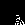
\includegraphics[width=0.1\textwidth]{images/amazon_2.png}\\
	\hline
	2 & 7 & 625 & 1,12\% & 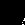
\includegraphics[width=0.1\textwidth]{images/facebook_2.png}\\
	\hline
	3 & 20 & 625 & 3,2\% & 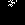
\includegraphics[width=0.1\textwidth]{images/google_2.png}\\
	\hline
	4 & 251 & 1089 & 23,05\% & 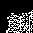
\includegraphics[width=0.1\textwidth]{images/hallo_3.png}\\
	\hline
	5 & 53 & 625 & 8,48\% & 
\includegraphics[width=0.1\textwidth]{images/reddit_1.png}\\	
	\hline
	6 & 11 & 625 & 1,76\% & 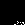
\includegraphics[width=0.1\textwidth]{images/reddit_2.png}\\	
	\hline
	7 & 28 & 441 & 6,35\% & 
\includegraphics[width=0.1\textwidth]{images/test1_2.png}\\	
	\hline
	8 & 12 & 441 & 2,72\% & 
\includegraphics[width=0.1\textwidth]{images/test2_2.png}\\	
	\hline
\end{tabular}
\caption{Teilweise richtig erkannte QR-Codes. Die weißen Pixel sind falsch erkannte Module.}
\label{tab:teilweiseKorrekt}
\end{table}

\newpage
\section{Fazit und Ausblick}
Zusammenfassend wurde das Ziel, planare QR-Codes unter perspektivischer Verzerrung zu erkennen, erreicht. Die Eingabebilder werden nach Positionsmarkern eines QR-Codes durchsucht. Sobald drei Positionsmarker gefunden wurden, wird die konvexe Hülle um diese Marker gebildet. Aus jeweils zwei der Eckpunkte der konvexen Hülle werden darauf folgend Gerade gebildet. Der Schnittpunkt dieser Geraden dient als vierter Eckpunkt des QR-Codes. Im nächsten Schritt erfolgt die geometrische Normalisierung mit anschließender Bestimmung der Modulgröße im Bild. Mit Hilfe der Modulgröße kann der QR-Code entsprechend den Anforderungen skaliert werden, sodass jedes Modul ein Pixel groß ist. Da zusätzlich eine Binarisierung stattfindet, enthält das Ausgabebild nur noch schwarze oder weiße Pixel. 

Während der Evaluierung wurden 62\% der QR-Codes komplett richtig erkannt, 32\% nur teilweise und 7\% überhaupt nicht. Ein Schwachpunkt liegt dabei in der Erstellung der Testbilder. Da die QR-Codes ausgedruckt wurden, wellt sich das Papier auf den Testbildern und ist dadurch nicht mehr planar. Da unser Programm für planare QR-Codes optimiert wurde, konnte so der vierte Punkt nicht mehr exakt bestimmt. Dies führt insbesondere im unteren rechten Bereich der QR-Codes zu Fehlern (siehe Tabelle \ref{tab:teilweiseKorrekt}). 

Die Ungenauigkeit bei der Bestimmung des vierten Eckpunktes ist generell ein Aspekt der Umsetzung, der noch Verbesserungspotential bietet. Der vierte Eckpunkt wird durch ein Schnittpunkt zweier Geraden bestimmt, welche durch je zwei Punkte definiert werden, die relativ nah aneinander liegen. Um eine exaktere Bestimmung zu ermöglichen, wäre es sinnvoll die Gerade durch weiter auseinander liegende Punkte zu ermitteln. Im aktuellen Ansatz der Implementierung ist die Erweiterung der konvexen Hülle auf schwarze Module im QR-Code eine Möglichkeit um dies zu erreichen.

In einem der Testbilder wurde außerdem der dünne schwarze Rahmen um die Sperrzone als Positionsmarker gekennzeichnet, was im Folgenden zu deutlichen Fehlern geführt hat. Dies liegt vermutlich an einer ungünstigen Schachtelung von Konturen im QR-Code und tritt äußerst selten auf. Durch weitere Überprüfungen bei der Bestimmung der Positionsmaker, durch beispielsweise Abgleichen der Konturformen zueinander, sollte dieser Fehler behoben werden können.

Das entwickelte Programm ist in der Lage QR-Codes unter perspektiver Verzerrung sowie bei Bildunschärfe, Rotations-, Belichtungs- und Skalierungsveränderungen zu erkennen. Die Codes werden in eine normalisierte Version transformiert, welche im nächsten Schritt durch ein Lesegerät lesbar wäre. Die Anwendung bietet dennoch Potential zur Verbesserung, wobei die exaktere Bestimmung des vierten Eckpunktes im Fokus liegt. Dadurch sollte die Anzahl der teilweise richtig erkannten QR-Codes zugunsten der komplett richtig erkannten Codes minimiert werden.


\newpage

\nocite{*}
\bibliographystyle{plain}
\bibliography{bib/literature}

\end{document}